%---------- Quinto Capítulo: Desenvolvimento do Software ----------
\chapter{Desenvolvimento do Software}
\label{chap:desenv}

Utilizando a metodologia e o projeto do sistema apresentados nos capítulos \ref{metod} e \ref{specs}, respectivamente, inicou-se o desenvolvimento efetivo do sistema.
Primeiramente foi criado um projeto Maven principal denominado \texttt{onibuscerto}, o qual foi dividido em quatro subprojetos: 
\begin{itemize}
	\item \texttt{onibuscerto-api}: contém a classe que representa coordenadas geográficas e o objeto resposta contendo informações da rota ao Cliente.
	\item \texttt{onibuscerto-core}: consiste no módulo \emph{Core} definido no projeto do software (seção \ref{specs}). 
	Contém as representações das entidades originárias dos arquivos GTFS e faz interface do sistema com o banco de dados.
	\item \texttt{onibuscerto-importer}: consiste no módulo \emph{Importer} definido no projeto do software (seção \ref{specs}).
	Responsável pela importação dos dados contidos nos arquivos GTFS para o sistema através das funcionalidades do \emph{Core}.
	\item \texttt{onibuscerto-service}: consiste nos módulos \emph{Web Service} e Cliente definidos na seção \ref{specs}. 
	Pretende-se futuramente separar este subprojeto em dois outros distintos representando tais módulos.
\end{itemize}

Nas subseções a seguir serão descritos detalhes a respeito da implementação de cada subprojeto.

\section{Configuração do ambiente de desenvolvimento}

\section{onibuscerto-core}

O \emph{Core} consiste basicamente na interface do sistema com o banco de dados, contendo portanto as representações das entidades originárias dos arquivos GTFS.
Estas representações nada mais são do que classes no sistema que são responsáveis pelo encapsulamento das entidades do banco de dados.
Cada uma destas classes foi implementada com o intuito de referenciar um nó ou aresta do grafo armazenado. 

O \emph{Core} foi organizado de tal forma que todas as suas classes de entidades possuam suas respectivas \emph{factories}.
Como já comentado, \emph{factory} consiste em uma interface com o objetivo de criação de famílias de objetos dependentes ou correlacionados.
Desta forma, toda criação de entidades é realizada através de uma \emph{factory}, centralizando este processo a somente uma classe por entidade.

Cada \emph{factory} é armazenada no banco de dados como um nó de referência, o qual possui uma relação para cada nó de sua respectiva entidade.
Esta organização das \emph{factories} no grafo pode ser observada na figura \ref{fig:grafoFactory}.

\begin{figure}[!htb]
	\centering
	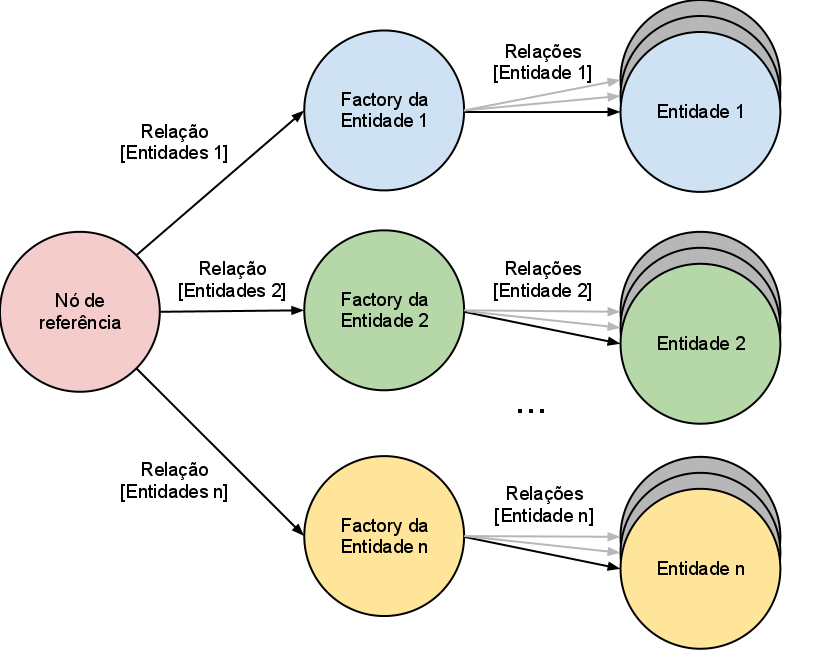
\includegraphics[width=0.7\textwidth]{./imgs/grafoFactory.png}
	\caption[Arquitetura do sistema]{Visão geral da organização das \emph{factories} do grafo.}
	\fonte{Autoria Própria}
	\label{fig:grafoFactory}
\end{figure}


%wrappers Neo4j
%entidades do banco de dados sao encapsuladas em classes no sistema, sendo que cada uma contem uma referencia a um nó ou uma aresta.
%essas entidades abstraem o acesso ao banco de dados, se precisar mudar é só mudar as factories.

\subsection{Entidades}

\subsubsection{Location}

\subsubsection{Stop}

\subsubsection{Route}

\subsubsection{Trip}

\subsubsection{StopTime}

\subsubsection{Connection}


\subsection{DatabaseController}


\section{onibuscerto-importer}

\section{onibuscerto-service}

O subprojeto \texttt{onibuscerto-service} é onde encontram-se os Servlets responsáveis por executar consultas na base de dados construída pelo \emph{Importer}.
Os Servlets funcionam sob a forma de \emph{web services} e, sendo assim, todas as consultas são requisitadas pelos clientes através de requisições \sigla{HTTP}{Hypertext Transfer Protocol} do tipo GET ou POST.
As implementações dos Servlets residem no pacote \texttt{com.onibuscerto.service.servlets}.

Atualmente, apenas consultas que determinam a rota com o menor tempo de viagem entre duas coordenadas geográficas estão implementadas.
O Servlet responsável por executar esse tipo de consulta está implementado na classe \texttt{RouteServlet}.
No início do seu ciclo de vida, este Servlet é responsável por obter uma instância da classe \texttt{DatabaseController} do \emph{Core}, a qual será utilizada para acessar o banco de dados e resolver as consultas.
Em seguida, assim como um Servlet comum, este muda para um estado no qual está disponível para atender requisições dos clientes.
Por fim, ao ser destruído, o \texttt{RouteServlet} deve chamar o método \texttt{close} do \texttt{DatabaseController}, com o objetivo de fechar a conexão com o banco de dados.
O ciclo de vida completo do Servlet é ilustrado na Figura \ref{fig:servletciclo}.

\begin{figure}[!htb]
	\centering
	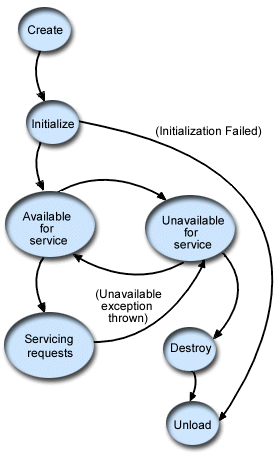
\includegraphics[width=0.4\textwidth]{./imgs/servletciclo.png}
	\caption[Ciclo de vida de um Servlet]{Ciclo de vida de um Servlet}
	\fonte{\citeonline{infocenter}}
	\label{fig:servletciclo}
\end{figure}

\section{Considerações}
